%%%%%%%%%%%%%%%%%%%%%%%%%%%%%%%%%%%%%%%%%
% Short Sectioned Assignment
% LaTeX Template
% Version 1.0 (5/5/12)
%
% This template has been downloaded from:
% http://www.LaTeXTemplates.com
%
% Original author:
% Frits Wenneker (http://www.howtotex.com)
%
% License:
% CC BY-NC-SA 3.0 (http://creativecommons.org/licenses/by-nc-sa/3.0/)
%
%%%%%%%%%%%%%%%%%%%%%%%%%%%%%%%%%%%%%%%%%

%----------------------------------------------------------------------------------------
%	PACKAGES AND OTHER DOCUMENT CONFIGURATIONS
%----------------------------------------------------------------------------------------

\documentclass[paper=a4, fontsize=11pt]{scrartcl} % A4 paper and 11pt font size

\usepackage[T1]{fontenc} % Use 8-bit encoding that has 256 glyphs
\usepackage{fourier} % Use the Adobe Utopia font for the document - comment this line to return to the LaTeX default
\usepackage[english]{babel} % English language/hyphenation
\usepackage{amsmath,amsfonts,amsthm} % Math packages

\usepackage{lipsum} % Used for inserting dummy 'Lorem ipsum' text into the template

\usepackage{sectsty} % Allows customizing section commands
\allsectionsfont{\centering \normalfont\scshape} % Make all sections centered, the default font and small caps

\usepackage{fancyhdr} % Custom headers and footers

% my packages
\usepackage{commath}
\usepackage{mathtools}
\usepackage{graphicx}
\DeclarePairedDelimiter{\ceil}{\lceil}{\rceil}

\pagestyle{fancyplain} % Makes all pages in the document conform to the custom headers and footers
\fancyhead{} % No page header - if you want one, create it in the same way as the footers below
\fancyfoot[L]{} % Empty left footer
\fancyfoot[C]{} % Empty center footer
\fancyfoot[R]{\thepage} % Page numbering for right footer
\renewcommand{\headrulewidth}{0pt} % Remove header underlines
\renewcommand{\footrulewidth}{0pt} % Remove footer underlines
\setlength{\headheight}{13.6pt} % Customize the height of the header

\numberwithin{equation}{section} % Number equations within sections (i.e. 1.1, 1.2, 2.1, 2.2 instead of 1, 2, 3, 4)
\numberwithin{figure}{section} % Number figures within sections (i.e. 1.1, 1.2, 2.1, 2.2 instead of 1, 2, 3, 4)
\numberwithin{table}{section} % Number tables within sections (i.e. 1.1, 1.2, 2.1, 2.2 instead of 1, 2, 3, 4)

\setlength\parindent{0pt} % Removes all indentation from paragraphs - comment this line for an assignment with lots of text

% new commands
\newcommand{\filename}[1]{\textbf{\textit{#1}}}
\newcommand{\funcname}[1]{\textbf{#1}}
\newcommand{\inv}{^{\raisebox{.2ex}{$\scriptscriptstyle-1$}}}
\renewcommand{\vec}[1]{\mathbf{#1}}

\DeclareMathOperator*{\argmin}{arg\,min} % Jan Hlavacek

%----------------------------------------------------------------------------------------
%	TITLE SECTION
%----------------------------------------------------------------------------------------

\newcommand{\horrule}[1]{\rule{\linewidth}{#1}} % Create horizontal rule command with 1 argument of height

\title{	
\normalfont \normalsize 
\textsc{Mathematical foundations of computer graphics and vision} \\ [25pt] % Your university, school and/or department name(s)
\horrule{0.5pt} \\[0.4cm] % Thin top horizontal rule
\huge Exercise 1. Robust Estimation and Optimization \\ % The assignment title
\horrule{2pt} \\[0.5cm] % Thick bottom horizontal rule
}

\author{Dongho Kang \\ \small 16-948-598} % Your name

\date{\normalsize March 12, 2017} % Today's date or a custom date

\begin{document}

\maketitle % Print the title

%----------------------------------------------------------------------------------------
%	README
%----------------------------------------------------------------------------------------

MATLAB R2016b version was used for coding and testing:

\begin{center}
MathWorks, MATLAB R2016b (9.1.0.441655) \\
64-bit (maci64) 
\end{center}

The \filename{code} directory contains followings:

\begin{itemize}
	\item \filename{part1.m} \quad Script .m file for part1.
	\item \filename{part2.m} \quad Script .m file for part2.
	\item \filename{functions dir} \quad Function .m files 
		\begin{itemize}
			\item \funcname{GenerateInlierData.m} \quad Function .m file for generating inliers.
			\item \funcname{GenerateOutlierData.m} \quad Function .m file for generating outliers.
			\item \funcname{VerifyInlier.m} \quad Function .m file for verifying inliers.
			\item \funcname{RansacForCircularModel.m} \quad Function .m file for RANSAC implementation.
			\item \funcname{ExhSearchForCircularModel.m} \quad Function .m file for exhaustive search.			
			\item \funcname{CircularModelFitting.m} \quad Function .m file for circular model fitting. 		
			\item \funcname{PlotBestRansacResult.m}  \quad Function .m file for plotting RANSAC result.			
			\item \funcname{Cost.m}	\quad Function .m file for calculating vertical cost.						
			\item \funcname{IRLSWithL1Norm.m} \quad Function .m file for IRLS with $L_{1}$ norm.
			\item \funcname{LinProgWithLqNorm.m} \quad Function .m file for LP with $L_{1}$ and $L_{\infty}$ norm. 							
		\end{itemize}
\end{itemize}

For running exercise parts, adjust several parameters and run the corresponding script on the MATLAB environment. More details are stated in the \textit{Running} section.

%----------------------------------------------------------------------------------------
%	PROBLEM 1
%----------------------------------------------------------------------------------------

\section{exercise part 1: ransac for circle fitting}

%----------------------------------------------------------------------------------------
%	DESCRIPTION
%----------------------------------------------------------------------------------------
\subsection{Description}

In exercise part 1, RANSAC algorithm was used for circular model fitting with $N$ number of 2D data points which were corrupted by noise and certain ratio of outliers. The implementation of part 1 corresponds to the .m script file \filename{part1.m} and the script consists of several parts which can be executed separately: 

\begin{itemize}
\item Data generation and verification
\item Running RANSAC algorithm for circular model fitting
\item Running exhaustive search for circular model fitting
\item Plotting the result
\end{itemize}  

%----------------------------------------------------------------------------------------
\subsubsection{Data generation and verification}

For certain outlier ratio $r  (\%)$ and $N$ number of 2D data points, the number of inliers ($n_{inlier}$)and outliers($n_{outlier}$) are as follows:

\begin{align*}
n_{inlier} &= N \times \frac{1 - r}{100}  \\
n_{outlier} &= N \times \frac{r}{100} 
\end{align*}

\begin{center}
$(N = 100$, $r \in \{5, 20, 30, 70\})$
\end{center}

In order to generate $n_{inlier}$ inliers and $n_{outlier}$ outliers, the function \funcname{GenerateInlierData} and \funcname{GenerateOutlierData} are implemented. \funcname{GenerateInlierData} generates noise-added data points with the inlier distance threshold $\tau = 0.1$ and \funcname{GenerateOutlierData} generates data points which of distance from the synthetic model are over the threshold $\tau$. It can be described as follows. $d\big(p_{1}, p_{2}\big)$ is euclidean distance function between two 2D points $p_{1}$ and $p_{2}$, $(x_{c}, y_{c})$ is the center of the synthetic circle and $R_{c}$ is the radius of the synthetic circle:

\begin{align*}
\abs{d \big( (x_{i}, y_{i}), (x_{c}, y_{c}) \big) - R_{c}} &\leq \tau  \qquad for (x_{i}, y_{i}) \in Set_{inlier} \\
\abs{d \big( (x_{j}, y_{j}), (x_{c}, y_{c}) \big) - R_{c}} &> \tau \qquad for (x_{j}, y_{j}) \in Set_{outlier} 
\end{align*}


After generating inliers and outliers, verified whether generated inliers follow the definition above. For this purpose, the function \funcname{VerifyInlier} is used. The specific descriptions for each steps are in the next page.

%----------------------------------------------------------------------------------------
\paragraph{Inlier generation}

A 2D point $(\tilde{x_{i}}, \tilde{y_{i}})$ on the circular model $(x-x_{c})^{2} + (y-y_c)^{2} = R_{c}^{2}$ which of center $(x_{c}, y_{c})$, and radius $R_{c}$ can be described as follows:

\begin{equation*}
(\tilde{x_{i}}, \tilde{y_{i}}) = (x_{c}, y_{c}) + R_{c} \times (\cos \theta_{i}, \sin \theta_{i}) \qquad \theta_{i} \in [0, 2 \pi], i = 1, 2, \dots n_{inlier}
\end{equation*}

Thus, picked $n_{inlier}$ number of random float numbers from the range of  $[0, 2 \pi]$ by MATLAB function \funcname{rand} and as using these numbers as $\theta_{i}$, generated $(x_{i}, y_{i})$ for $i = 1, 2, \dots n_{inlier}$.  

Random noise $(\sigma_{x_{i}}, \sigma_{y_{i}})$ is added on the data point $(\tilde{x_{i}}, \tilde{y_{i}})$ as follows:

\begin{equation*}
(x_{i}, y_{i}) = (\tilde{x_{i}}, \tilde{y_{i}}) + (\sigma_{x_{i}}, \sigma_{y_{i}}) 
\quad s.t. \quad \sigma_{x_{i}}, \sigma_{y_{i}} \in [-0.1, 0.1], \quad \abs{d \big( (x_{i}, y_{i}), (x_{c}, y_{c}) \big) - R_{c}} \leq \tau 
\end{equation*}

To implement this, two random float numbers by \funcname{rand} were picked for $(\sigma_{x_{i}}, \sigma_{y_{i}})$ iteratively, until it satisfies $\abs{d \big( (x_{i}, y_{i}), (x_{c}, y_{c}) \big) - R_{c}} \leq \tau$ and repeated it for $i=1,\dots,n_{inlier}$ to generate $n_{inlier}$ number of inliers. Also, $(x_{i}, y_{i})$ is checked whether it is in the domain $[-10, 10]$.

%----------------------------------------------------------------------------------------
\paragraph{Outlier generation}

In order to generate one outlier point $(x_{j}, y_{j})$, two random float numbers were generated by \funcname{rand} in the domain of $[-10, 10] \times [-10, 10]$ and generated $(x_{j}, y_{j})$ was checked whether it satisfies $\abs{d((x_{j}, y_{j}), (x_{c}, y_{c})) - R_{c}} > \tau$. If not, generated $(x_{j}, y_{j})$ again. Repeated this for $n_{outlier}$ times to generate $n_{outlier}$ number of outliers.

%----------------------------------------------------------------------------------------
\paragraph{Data verification}

Checked whether synthesized inliers are indeed inliers and outliers are indeed outliers. The function \funcname{VerifyInlier} was used. The function calculates $\abs{d((\tilde{x}_{i}, \tilde{y}_{i}), (x_{c}, y_{c})) - R_{c}}$ for each data points and check if there is a inlier point which of $\abs{d((x_{i}, y_{i}), (x_{c}, y_{c})) - R_{c}} > \tau$ or an outlier point which of $\abs{d((x_{j}, y_{j}), (x_{c}, y_{c})) - R_{c}} \leq \tau$. In this case, error is returned and the script halts. 

%----------------------------------------------------------------------------------------
\subsubsection{RANSAC for circular model fitting}

For generated data point $(x_{i}, y_{i})$ $i \in {1,2\dots,N}$, RANSAC algorithm applied to get the best model parameter which of maximum number of inliers within $n_{iter}$ RANSAC iterations.

\funcname{RansacForCircularModel} was implemented for RANSAC algorithm and the algorithm is applied for 1000 times for each outlier ratio to find the distribution of the number of inliers found by RANSAC. 
 \\

The number of RANSAC iterations $n_{iter}$ for success rate $p$ ($0 \leq p < 1$, for this exercise, $p = 0.99$), outlier ratio $r  (\%)$ and sample size $s$ ($=3$ for circular model: two for x, y coordinates of center and one for radius) is defined as follows: 

\begin{equation*}
n_{iter} = \ceil{ \frac{log(1 - p)}{log(1 - (1 - \frac{r}{100}) ^ {s})} }
\end{equation*}

Thus, $n_{iter} = 3$ for $r = 5\%$, $n_{iter} = 7$ for $r = 20\%$, $n_{iter} = 11$ for $r = 30\%$ and $n_{iter} = 169$ for $r = 70\%$. During $n_{iter}$ iterations, found the best result of RANSAC which of maximum number of inliers. \\

For each RANSAC iteration, sampled $s = 3$ data points without replacement. If the same data points are sampled, model fitting could be failed because it is under-determined problem. 

\paragraph{Circular model fitting}

With respect to sampled data points $(x_{1}', y_{1}'), (x_{2}', y_{2}'), (x_{3}', y_{3}')$, used \funcname{CircularModelFitting} for model fitting. The function solves the following equation (variables $a, b, c$ are parameter for fitted model which correspond to $x_c, y_c$ and $R_c$ for each):

\begin{align*}
(x_{1}' - a)^{2} + (y_{1}' - b)^{2} &= c^{2} \\
(x_{2}' - a)^{2} + (y_{2}' - b)^{2} &= c^{2} \\
(x_{3}' - a)^{2} + (y_{3}' - b)^{2} &= c^{2}
\end{align*}

As eliminating variable $c$, the equation can be expressed to linear equation as follows:

% A = [-2(x1 - x2), -2(y1 - y2); -2(x2 - x3), -2(y2 - y3)]
% B = [x2^2 - x1^2 + y2^2 - y1^2; x3^2 - x2^2 + y3^2 - y2^2]

\begin{equation*}
\begin{bmatrix}
    -2(x_{1}' - x_{2}')       &     -2(y_{1}' - y_{2}') \\
    -2(x_{2}' - x_{3}')       &     -2(y_{2}' - y_{3}') 
\end{bmatrix}
\begin{bmatrix}
    a \\
    b
\end{bmatrix}
=
\begin{bmatrix}
    x_{2}'^{2} - x_{1}'^{2} +  y_{2}'^{2} - y_{1}^{2} \\
    x_{3}'^{2} - x_{2}'^{2} +  y_{3}'^{2} - y_{2}^{2}
\end{bmatrix}
\end{equation*}

For $Ax = b$, if $A$ is square matrix and not singular then $x = A \inv b$. Thus $x = [a \quad b]^{T}$ can be obtained and after that, c also be calculated by the following equation: 

\begin{equation*}
c = \sqrt{x_{1}^{2} - 2 a x_{1} +  a^{2} + y_{1}^{2} - 2 b y_{1} + b^{2}}
\end{equation*}

As $a, b$ and $c$ (center and radius of the fitted circle) have been determined, set of inliers and outliers can be determined as being done for data verification. This circular model fitting algorithm can be used for not only RANSAC but also for exhaustive search algorithm.

%----------------------------------------------------------------------------------------
\subsubsection{Exhaustive search}

Another option for model fitting is trying every combination of data points and choosing the best combination. In order to do this, MATLAB function \funcname{nchoosek} was used. For $N = 100$ and $s = 3$, the number of all possible combination is as follows:

\begin{equation*}
n_{comb} = \binom{100}{3}=\frac{100!}{3! \times 97!}=161700
\end{equation*}

For each combination, used \funcname{CircularModelFitting} for model fitting and found the number of inliers of the fitted model. Finally, as compared result of each combinations, the best result of exhaustive search can be obtained. This was implemented as the function \funcname{ExhSearchForCircularModel}.

%----------------------------------------------------------------------------------------
%	RUNNING
%----------------------------------------------------------------------------------------
\subsection{Running}

Several parameters can be changed for running the script but only changing model parameters (i.e. variables x\_c, y\_c, radius, noise\_radius) is allowed to guarantee proper execution. If model parameter combination is not feasible(e.g. out of domain bound), error is returned. \\

%----------------------------------------------------------------------------------------
%	RESULT
%----------------------------------------------------------------------------------------
\subsection{Result}

\noindent\makebox[\textwidth]{
  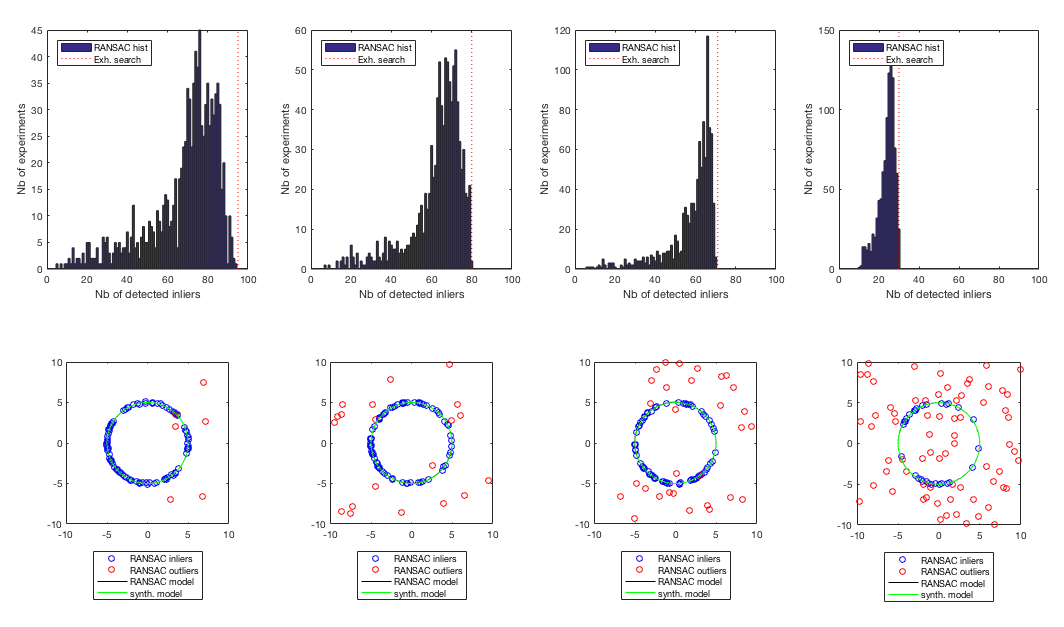
\includegraphics[width=0.8\paperwidth]{part1_plot_low}
}

The result of RANSAC circular fitting with different outlier ratios is as the plot above. The red lines on the histogram indicate the result of exhaustive search. (here the synthetic model is $center = (0, 0)$ and $radius = 5$)\\

The table shows the number of inliers and outliers of the fitted model by 1000 times of RANSAC test:

\begin{center}
    \begin{tabular}{ | c | c | c | c | c |}
    \hline
    $r$			&	5\%	&	20\%	&	30\%	&	70\% \\ \hline
    max. \# of inliers		&	94 		& 	80 		& 	70	& 	30 	\\ \hline
    avg. \# of intlier 		& 	68.13	& 	62.71 	& 	57.96	& 	23.88 \\ \hline
    std. \# of intlier 		& 	17.74	& 	13.13 	& 	11.87	& 	4.10 \\ \hline
    median. \# of intlier 	& 	73		& 	66 		& 	62		& 	25 \\ \hline
    \end{tabular}
\end{center} 

The table shows the number inliers and outliers of the best circular model by exhaustive search:

\begin{center}
    \begin{tabular}{ | c | c | c | c | c |}
    \hline
    $r$			&	5\%	&	20\%	&	30\%	&	70\% \\ \hline
    \# of inliers		&	95 	& 	80 	& 	71	& 	30 	\\ \hline
    \end{tabular}
\end{center} 

The table shows the average running time of RANSAC and the running time of exhaustive search:

\begin{center}
    \begin{tabular}{ | c | c | c | c | c |}
    \hline
    $r$			&	5\%	&	20\%	&	30\%	&	70\% \\ \hline
    RANSAC (avg.)	&	0.0028	&	0.0039	&	0.0060	&     0.0762	\\ \hline
    exh. search		&	62.10 	& 	55.73 	& 	57.94	& 	60.12 	\\ \hline
    \end{tabular}
\end{center} 

%----------------------------------------------------------------------------------------
%	DISCUSSION
%----------------------------------------------------------------------------------------
\subsection{Discussion}

Comparing RANSAC and exhaustive search:

\begin{itemize}
\item For $N = 100$:
    \begin{itemize}
        \item The number of combinations for $N = 100$ 
            \begin{equation*}
            n_{comb} = \binom{100}{3}=\frac{100!}{3! \times 97!}=161700
            \end{equation*}
        \item The number of RANSAC iterations for each outlier ratio for $N = 100$
            \begin{equation*}
            n_{iter} = \ceil{ \frac{log(1 - p)}{log(1 - (1 - \frac{r}{100}) ^ {s})} }
            \end{equation*}
            \begin{center}
                \begin{tabular}{ | l | l | l | l | l | }
                \hline
                $r =$ & 5\% & 20\% & 30\% & 70\% \\ \hline
                $n_{iter} = $ & 3 & 7 & 11 & 169 \\ \hline
                \end{tabular}
        \end{center}
        Thus, \textbf{running time of RANSAC increases as $r$ goes up.}
	\end{itemize}
\item For $N= 100,000$:
	\begin{itemize}
            \item The number of combinations for $N = 100,000$ 
            \begin{equation*}
            n_{comb} = \binom{100000}{3}=\frac{100000!}{3! \times 99997!}=166661666700000
            \end{equation*}
            \item The number of RANSAC iterations for $N = 100,000$ is same as the case of $N = 100$. \textbf{The number of RANSAC iteration is regardless of the size of data set.}
	\end{itemize}
\item The number of inlier of the best model searched by exhaustive search is always bigger (or equal) than RANSAC result.
	\begin{itemize}
		\item It because, exhaustive search tries all combinations of data points, and can find global optimal solution. 
		\item \textbf{RANSAC can only find local optimal solutions.}
		\item Nevertheless, the best result of 1000 RANSAC tests are close with the result of exhaustive search.
	\end{itemize}
\item The running time of exhaustive search and RANSAC:
	\begin{itemize}
		\item The running time is proportion of the number of iteration. Thus \textbf{RANSAC is much faster than exhaustive search.}
		\item However, as $r$ goes up, the number of RANSAC iteration also increases. Besides, the running time of exhaustive search is regardless of $r$.
	\end{itemize}
\item \textbf{In order to get a global optimal solution, RANSAC algorithm should be reapplied for several times, however it can be still faster than exhaustive search.} Although $n_{iter}$ of RANSAC increases as $r$ increases, since standard deviation of the number of inlier distribution decreases, the number of reapplying RANSAC ($n_{test}$) also can be decreased to save the total running time. 
\end{itemize}

%----------------------------------------------------------------------------------------
%	PROBLEM 2
%----------------------------------------------------------------------------------------

\section{exercise part 2: IRLS and norms for line fitting}

%----------------------------------------------------------------------------------------
%	DESCRIPTION
%----------------------------------------------------------------------------------------
\subsection{Description}

In exercise part 2, IRLS and Linear Programming algorithm was used for line model fitting with $N$ number of 2D data points which were corrupted by noise and certain ration of outliers. The implementation of part 2 corresponds to the .m script file \filename{part2.m} and the script consists of several parts: 

\begin{itemize}
\item Data generation and verification
\item Run IRLS with $L_{1}$ norm
\item Run LP with $L_{1}$ norm 
\item Run LP with $L_{\infty}$ norm 
\item Plot the result
\end{itemize}  

%----------------------------------------------------------------------------------------
\subsubsection{Data generation and verification}

To generate data points on the synthetic model line, the new cost function(vertical cost: \funcname{Cost}) was used instead of euclidean distance function. For data point $(x_{i}, y_{i})$ and line model $y = ax + b$, it was defined as follows:

\begin{equation*}
d\big((x_{i}, y_{i}), (a, b)\big) = \abs{y_{i} - (ax_{i} + b)}
\end{equation*}

Thus, inliers and outliers are defined as  follows:

\begin{align*}
d \big( (x_{i}, y_{i}), (a, b) \big) &\leq \tau  \qquad for (x_{i}, y_{i}) \in Set_{inlier} \\
d \big( (x_{j}, y_{j}), (a, b) \big) &> \tau \qquad for (x_{j}, y_{j}) \in Set_{outlier} 
\end{align*}

The strategy of data generation is almost same as exercise part 1 but line model and the new cost are adapted.

%----------------------------------------------------------------------------------------
\paragraph{Inlier generation}

A 2D point $(\tilde{x_{i}}, \tilde{y_{i}})$ on the line model $y = ax + b$ can be described as follows:

\begin{equation*}
\tilde{y_{i}} = a\tilde{x_{i}} + b \qquad \tilde{x_{i}} \in [-10, 10]
\end{equation*}

Random noise $(\sigma_{x_{i}}, \sigma_{y_{i}})$ is added on the data point $(\tilde{x_{i}}, \tilde{y_{i}})$ as follows:

\begin{equation*}
(x_{i}, y_{i}) = (\tilde{x_{i}}, \tilde{y_{i}}) + (\sigma_{x_{i}}, \sigma_{y_{i}}) \quad
s.t. \quad \sigma_{x_{i}}, \sigma_{y_{i}} \in [-0.1, 0.1], \quad d \big( (x_{i}, y_{i}), (a, b) \big) \leq \tau 
\end{equation*}


%----------------------------------------------------------------------------------------
\paragraph{Outlier generation}

An outlier point $(x_{j}, y_{j})$ is generated by two random float numbers and should be in the domain of $[-10, 10] \times [-10, 10]$ Also it is checked whether it satisfies $d \big( (x_{j}, y_{j}), (x_{c}, y_{c}) \big) > \tau$. 

%----------------------------------------------------------------------------------------
\paragraph{Data verification}

Inliers and outliers are verified whether satisfies the following conditions:
\begin{align*}
d \big( (x_{i}, y_{i}), (a, b) \big) &\leq \tau  \qquad for (x_{i}, y_{i}) \in Set_{inlier} \\
d \big( (x_{j}, y_{j}), (a, b) \big) &> \tau \qquad for (x_{j}, y_{j}) \in Set_{outlier} 
\end{align*}

%----------------------------------------------------------------------------------------
\subsubsection{IRLS with $L_{1}$ norm}

For model parameter $\vec{x} = (a, b)^{T}$ and data $\vec{y}_{i} = (x_{i}, y_{i})^{T}$ for $i = 1, 2 \dots\ N$, the line fitting problem can be expressed with $L_{1}$ norm:

\begin{gather*}
\argmin_{\vec{x}} C_{\rho}(\vec{x}) \\ 
where \quad C_{\rho}(\vec{x}) = \sum_{i=1}^{N} \rho \circ f_{i}(\vec{x}) = \sum_{i=1}^{N} d(\vec{y}_{i}, \vec{x}) \\
\end{gather*}

The form above can be changed to weighted least squares problem as defining $f_{i}(\vec{x}) = d(\vec{y}_{i}, \vec{x})^{2}$ and $\rho(s) = \sqrt{s}$ and was solved by IRLS(Iteratively Reweighted Least Squares):

\begin{gather*} 
\vec{x}^{t+1} = \argmin_{\vec{x}} C(\vec{x}, \vec{w}^{t}) = \argmin_{\vec{x}} \sum_{i=1}^{N}w_{i}^{t}f_{i}(\vec{x}) \\ 
where \quad w_{i}^{t} = \frac{1}{2}d(\vec{y}_{i}, \vec{x}^{t})^{-1}
\end{gather*}

In the function \funcname{IRLSWithL1Norm}, the problem was described as linear equation:

\begin{gather*} 
\vec{x}^{t+1} = \argmin_{\vec{x}} C(\vec{x}, \vec{w^{t}}) = \argmin_{\vec{x}} \sum_{i=1}^{n}w_{i}^{t}f_{i}(\vec{x}) 
	= \argmin_{\vec{x}}(A\vec{x} - b)^{T} W^{t} (A\vec{x} - b) = (A^{T}W^{t}A)\inv A^{T}W^{t}b\\
where \\
W^{t} = diag({w_{1}^{t}, w_{2}^{t}, \dots, w_{N}^{t}}), 
\quad 
A = 
\begin{bmatrix}
    x_{1}	&	1 \\
    x_{2}	&	1 \\
    \vdots	& \vdots	\\
    x_{N}	&	1
\end{bmatrix},
\quad b = 
\begin{bmatrix}
    y_{1}	\\
    y_{2}	\\
    \vdots	\\
    y_{N}
\end{bmatrix}
\end{gather*}

As iterating until $\norm{\vec{x}^{t+1} - \vec{x}^{t}} < tol$ ($tol$ is an error tolerance), $\vec{x} = (a, b)^{T}$ can be obtained.

\pagebreak

%----------------------------------------------------------------------------------------
\subsubsection{LP with $L_{1}$ norm }

The line fitting problem with $L_{1}$ norm: 

\begin{gather*}
\argmin_{\vec{x}} \sum_{i=1}^{N} d(\vec{y}_{i}, \vec{x}) = \argmin_{\vec{x}} \norm{A\vec{x} - b}_{1}  = 
\argmin_{\vec{x}} \sum_{i=1}^{N} \abs{A_{i}\vec{x} - b_{i}} \\
where \\
A_{i} = 
\begin{bmatrix}
    x_{i}	&	1 
\end{bmatrix},
\quad b_{i} = 
\begin{bmatrix}
    y_{i}	
\end{bmatrix}
\end{gather*}

It can be solved by linear programming algorithm:

\begin{gather*}
\min_{\vec{x}, t_{1}, \dots, t_{N}} \sum_{i=1}^{N} t_{i} \\
 s.t. \quad \abs{A_{i}\vec{x} - b_{i}} \leq t_{i}, \quad i = 1, \dots, N
\end{gather*}

The MATLAB function \funcname{linprog(A, b, f)} can be used:

\begin{gather*}
\textbf{A} = \left[
\begin{array}{c|c}
    \begin{array}{c c}
        -x_{1}	&	-1\\
        -x_{2}	&	-1\\
        \vdots	& \vdots \\
        -x_{N}	&	-1
    \end{array}
    &
    - \mathbb{1}_{N \times N} \\
    \hline
    \begin{array}{c c}
        x_{1}	&	1\\
        x_{2}	&	1\\
        \vdots	& \vdots \\
        x_{N}	&	1
    \end{array}
    &
    - \mathbb{1}_{N \times N} 
\end{array} \right],
\quad \textbf{b} = \left[
\begin{array}{c}
    -y_{1}	\\
    -y_{2}	\\
    \vdots	\\
    -y_{N}	\\
    \hline	
    y_{1}	\\
    y_{2}	\\
    \vdots	\\
    y_{N}
\end{array} \right], 
\quad \textbf{f} = 
    \begin{bmatrix}
    0\\
    0\\
    1\\
    \vdots	\\
    1
    \end{bmatrix}, 
\quad \textbf{x'} = 
    \begin{bmatrix}
    a\\
    b\\
    t_{1}\\
    \vdots	\\
    t_{N}
    \end{bmatrix}
\end{gather*}

As \funcname{linprog(A, b, f)} solves $\min_{\textbf{x'}} \textbf{f}^{T} \textbf{x'}$ such that $\textbf{A x} \leq \textbf{b}$, the line parameter $\vec{x} = (a, b)^{T}$ can be obtained from \textbf{x'}.

%----------------------------------------------------------------------------------------
\subsubsection{LP with $L_{\infty}$ norm}

The line fitting problem with $L_{\infty}$ norm: 

\begin{gather*}
\argmin_{\vec{x}} \norm{A\vec{x} - b}_{\infty}  = 
\argmin_{\vec{x}} \max_{i = 1, \dots, N} \abs{A_{i}\vec{x} - b_{i}} \\
where \\
A_{i} = 
\begin{bmatrix}
    x_{i}	&	1 
\end{bmatrix},
\quad b_{i} = 
\begin{bmatrix}
    y_{i}	
\end{bmatrix}
\end{gather*}

\pagebreak

It can be solved by linear programming algorithm:

\begin{gather*}
\min_{\vec{x}, t} t \\
 s.t. \quad \abs{A_{i}\vec{x} - b_{i}} \leq t, \quad i = 1, \dots, N
\end{gather*}

Thus, \textbf{A}, \textbf{B}, \textbf{f} and \textbf{x'} for \funcname{linprog(A, b, f)} are as follows:

\begin{gather*}
\textbf{A} = \left[
\begin{array}{c}
    \begin{array}{c c c}
        -x_{1}	&	-1	&	-1\\
        -x_{2}	&	-1	&	-1\\
        \vdots	& \vdots	&	\vdots \\
        -x_{N}	&	-1	&	-1
    \end{array} \\
    \hline 
    \begin{array}{c c c}
        x_{1}	&	1	&	-1\\
        x_{2}	&	1	&	-1\\
        \vdots	& \vdots	&	\vdots \\
        x_{N}	&	1	&	-1
    \end{array}
\end{array} \right],
\quad \textbf{b} = \left[
\begin{array}{c}
    -y_{1}	\\
    -y_{2}	\\
    \vdots	\\
    -y_{N}	\\
    \hline	
    y_{1}	\\
    y_{2}	\\
    \vdots	\\
    y_{N}
\end{array} \right], 
\quad \textbf{f} = 
    \begin{bmatrix}
    0\\
    0\\
    1
    \end{bmatrix}, 
\quad \textbf{x'} = 
    \begin{bmatrix}
    a\\
    b\\
    t
    \end{bmatrix}
\end{gather*}

The line parameter $\vec{x} = (a, b)^{T}$ can be obtained from \textbf{x'}

%----------------------------------------------------------------------------------------
%	RUNNING
%----------------------------------------------------------------------------------------
\subsection{Running}

Only changing model parameters (i.e. variables a, b and noise\_radius) is allowed to guarantee proper execution. If the model parameter combination is not feasible(e.g. out of domain bound), error would be returned. \\

%----------------------------------------------------------------------------------------
%	RESULT
%----------------------------------------------------------------------------------------
\subsection{Result}

\noindent\makebox[\textwidth]{
  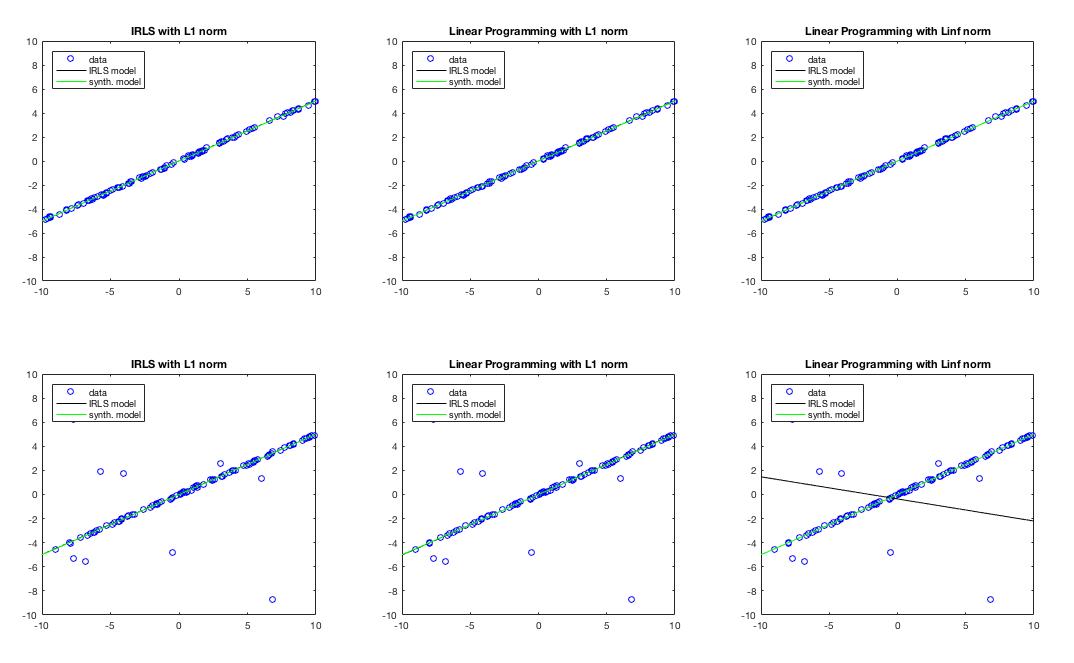
\includegraphics[width=0.8\paperwidth]{part2_plot_low}
}

The result of IRLS with $L_{1}$ norm, LP with $L_{1}$ norm and LP with $L_{\infty}$ for line fitting with different outlier ratios is as the plot above. The synthetic line model is $y = \frac{1}{2}x$.\\

The table shows the parameters and total cost for the data set of the fitted line model:

\begin{center}
    \begin{tabular}{ | c | c | c | c |}
    \hline
    $r$			&	0\%				&	0\%				&	0\%				 \\ \hline
    algorithm		&	IRLS	 with $L_{1}$	&	LP	 with $L_{1}$	&	LP with $L_{\infty}$		\\ \hline	
    fitted model		&	(0.5015, 0.0069) 	& 	(0.5010, 0.0118) 	& 	 (0.5006, -0.0018)	\\ \hline
    cost 			& 	2.1312			& 	4.2592 			& 	0.09517			 \\ \hline
    \end{tabular}
\end{center} 

\begin{center}
    \begin{tabular}{ | c | c | c | c |}
    \hline
    $r$			&	10\%				&	10\%				&	10\%				 \\ \hline
    algorithm		&	IRLS	 with $L_{1}$	&	LP	 with $L_{1}$	&	LP with $L_{\infty}$		\\ \hline	
    fitted model		&	(0.4996, 0.0128) 	& 	(0.5026, 0.0026) 	& 	(-0.1835, -0.3687)	\\ \hline
    cost 			& 	29.3508			& 	58.573 			& 	7.0647			 \\ \hline
    \end{tabular}
\end{center} 


%----------------------------------------------------------------------------------------
%	DISCUSSION
%----------------------------------------------------------------------------------------
\subsection{Discussion}

Comparing IRSL with $L_{1}$, LP with $L_{1}$ and LP with $L_{\infty}$:

\begin{itemize}
\item For $r = 0$, three algorithms shows equally good results. 
\item For $r = 10$, \textbf{algorithms using $L_{1}$ norm are robust to outliers but $L_{\infty}$ is not.}
	\begin{itemize}
		\item Using $L_{\infty}$, optimization algorithm(here, LP) tries to minimize only maximum value of $d(\vec{y}_{i}, \vec{x})$ i.e. it over-penalizes outliers.
		\item Over-penalizing tends to be worse as using $L_{q}$ norm with larger $q$.
	\end{itemize} 
\item Concerning running time, tried to check running time of each algorithms with $r = 0, 10, 70$ and the result is as follows:

\begin{center}
    \begin{tabular}{ | c | c | c | c |}
    \hline
    $r$				&	0\%				&	10\%				&	70\%				 \\ \hline
    IRLS with $L_{1}$		&	0.02116			&	0.027398			&	0.056931		\\ \hline	
    LP	 with $L_{1}$		&	1.3543 			& 	0.38858		 	& 	0.25859		\\ \hline
    LP with $L_{\infty}$ 	& 	0.34789			& 	0.22952 			& 	0.19325		 \\ \hline
    \end{tabular} \\
\end{center}  

    For line fitting problem, IRLS converges fast even for high value of $r$.
\end{itemize}


%----------------------------------------------------------------------------------------

\end{document}